The main goal of the thesis is to propose an approach which will be able to create the graphical overviews of critical business data and make decisions based on them. This chapter describes each part of the proposed approach. The chapter is divided to these parts:	
    \begin{enumerate}
      \item Which kind of data the application collects and how works with them.
      \item How real-time process visualization is done.
      \item What kind of overviews the application can display. 
    \end{enumerate}
% -----------------------------------------------------------------------
\section{Business Data Aggregation}
Each enterprise system collects precious data within business. These data are important in many ways. One is for business analysts. Analyst can with these collected data analyse processes and optimize them. Although every enterprise solution has differently defined structure of these data and every \gls{bpms} has different approach how it works with them, the core concept of how data can be described remains the same. 
Within \gls{bpms} there are elements which can be transformed always to the \gls{demo} concepts.
\begin{itemize}
\item There are always some kind of \textit{Actor roles} and concrete \textit{Actors}. Commonly \gls{bpms} defines \textit{Actor roles} as ``roles'' and \textit{Actors} defines as ``users''.
\item The processes itself can be transformed to \textit{Transactions}. In~\cref{ch:theoretical-foundations} was explained that each process can be described on ontological level and has precise definition what kind of process it is and the responsibilities of \textit{Actors}.
\item Each \gls{bpms} provides some kind of events, which can be used to determine what exactly happened and how it is connected to the model defined within \gls{demo}.
\end{itemize}

\begin{figure}[ht!]
  \centering
  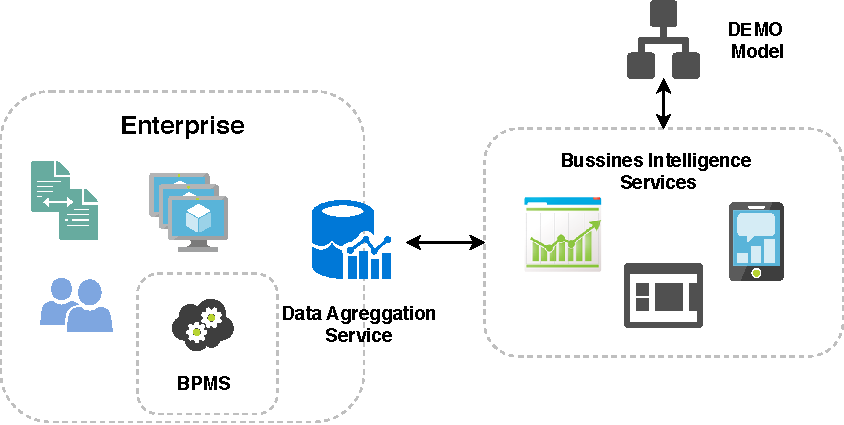
\includegraphics[width=12cm,keepaspectratio]{img/bi-demo-overview}
  \caption{Business Intelligence based on DEMO}
  \label{fig:bi-demo-overview}
\end{figure}    

In this way the system of visualisation based on \gls{demo} can be nearly independent from other systems within enterprise. The architecture of Business Intelligence based on \gls{demo} is shown at~\cref{fig:bi-demo-overview}. The enterprise does not need necessary a \gls{bpms}. Within enterprise, many systems and applications exists. Even without BPMS solutions within enterprise there are still the same kind of processes and actor roles which can be modelled through \gls{demo}.

Inside an enterprise there can be many systems and (not necessary) in front of them can be a \gls{bpm} solution. On the ``borders'' of the \textit{Enterprise} is placed \textit{Data Aggregation Service}. This service has responsibility of getting data from an \textit{Enterprise} and transforming them to the structure that \textit{Business Intelligence Services} can use. Collected data from \textit{Data Aggregation Service} are mapped to defined \textit{DEMO Model}.
With this approach, \textit{Business Intelligence Services} can take advantages of \gls{demo} without requirement to be dependent directly on enterprise systems.
% ----------------------------------------------------------------------------------------
\subsection{Business Data Domain Model}
\begin{figure}[ht!]
  \centering
  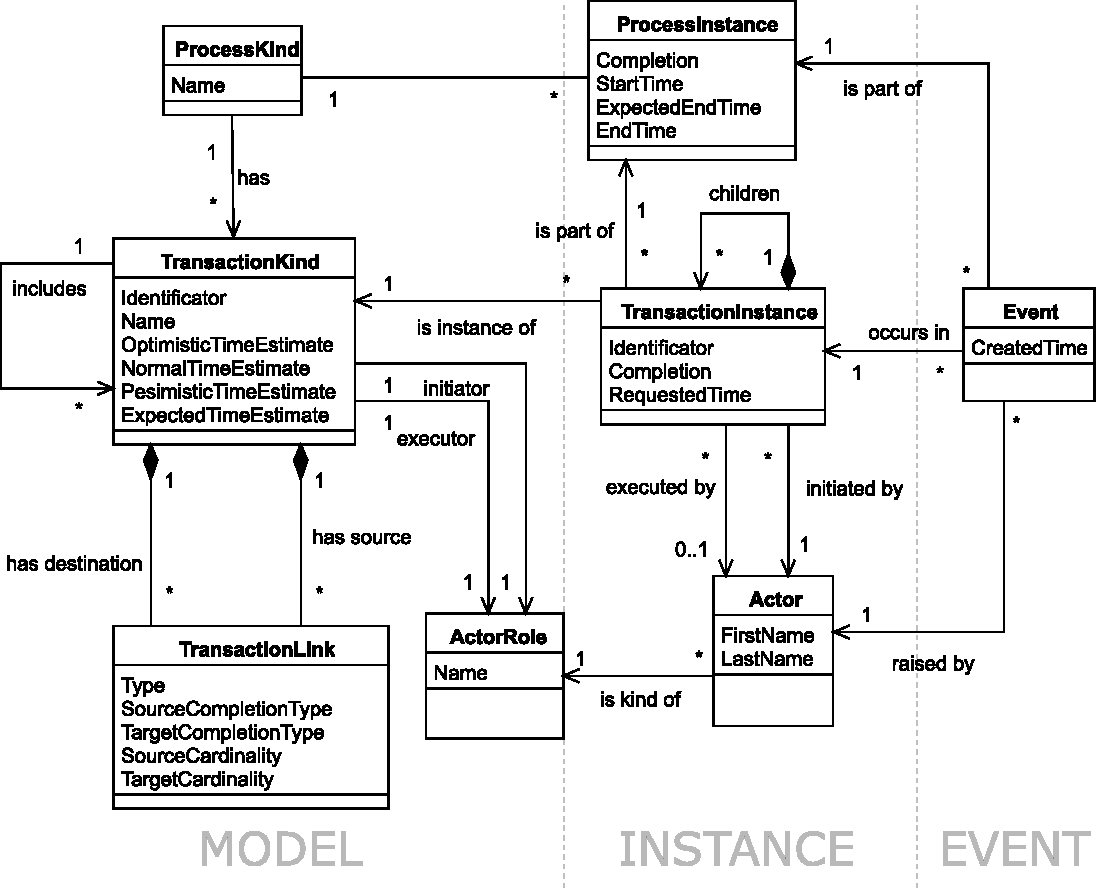
\includegraphics[width=13cm,keepaspectratio]{img/domain-data-model}
  \caption{Domain model of collected data}
  \label{fig:domain-data-model}
\end{figure}    

The one of the most important thing what needs to be defined is how collected data can be expressed for visualisation. The \cref{fig:domain-data-model} shows domain-data model which describes how \gls{demo} model can be described.  

\Cref{fig:domain-data-model} is divided to three parts:
\begin{description}
\item[Model] -- Defines how \gls{demo} model can be described. It corresponds with \gls{ocd} and \gls{psd} models.
\item[Instance] -- The one concrete running process. It indicates state of transactions. 
\item[Event] -- Last part defines the concrete occurred events from internal systems which can be collected and transformed to data, that can be used. 
\end{description}

The brief explanation of each entity from domain model:
\begin{description}
\item[Actor Role] -- Defines role within enterprise. 
\item[Actor] -- Defines concrete user within enterprise, which has assigned \textit{Actor Role}.

\item[Process Kind] -- Defines exactly one concrete business process inside enterprise. Each \textit{Process Kind} has linked amount of \textit{Transaction Kinds}.

\item[Process Instance] -- The instance of concrete \textit{Process Kind}. Defines process \textit{Completion}, date when process instance was created (\textit{StartTime}) and expected time when whole process will be completed (\textit{ExpectedEndTime}).

\item[Transaction Kind] -- Defines the transaction kind. It has linked information, which \textit{Actor Role} is initiator or executor respectively. Also defines the time estimates for transaction completion. These three time estimates -- \textit{Optimistic}, \textit{Normal}, \textit{Pessimistic} are used to compute real expected time. 

\item[Transaction Link] -- Defines the \textit{response} or \textit{waiting} links. Each link has defined \textit{target Transaction Kind}  and \textit{source Transaction Kind} to determine which two \textit{Transaction Kinds} link connects. Link also defines \textit{Source Cardinality} and \textit{Target Cardinality} to define cardinalities. Moreover link defines which \textit{C-Act} is assigned to source and target transactions.  

\item[Transaction Instance] -- Each \textit{Transaction Kind} could have more than one instance. Transaction Instance includes information about \textit{Completion} and \textit{Requested Time}. The instance itself could have more than one children. 

\item[Event] -- An entity to define events which can occur during the running process. Each event has time creation (\textit{Created}) and duration how long it take to between last event and before event was created.

% \item[Completion Changed Event] Event which describes that some C-Act happened within transaction. 
% \item[Initiator / Executor Event] Events which describe that initiator or executor were assigned to \textit{Transaction Instance}. In other words, \textit{Transaction Instance} was initiated or executed by given initiator or executor respectively.
\end{description}
% ---------------------------------------------------------------------------------------

\subsection{A Time Estimate Computation}
Each \textit{Transaction Kind} has three time attributes -- \textit{Optimistic}, \textit{Normal}, \textit{Pessimistic} time estimate. Each one indicates how quickly given task could be completed. These attributes are set manually and it is important decision which values are given. From this three attributes the resulting one is computed.  

Computation is done through technique \textit{Three Point Estimation} \cite{beta-distribution}. 
Manager can take simple average of this three attributes, however the weighted average is more precise.
The following formula comes from \textit{Beta distribution} also known as \textit{PERT}:

\begin{displaymath}
\centering
ExpectedTimeEstimate = \frac{O + 4*N + P}{6}
\end{displaymath}
where (O) states for optimistic, (N) for normal and (P) for pessimistic estimates. It indicates that normal estimate ``can happen'' most likely.
% ----------------------------------------------------------------------------------------
\section{Case Study Rent-A-Car}
Although all proposed approaches are defined generally, the case study is used to demonstrate usage and show examples. The case study is taken from book by J.Dietz~\cite{dietz-essence-2015}. A Rent-A-Car is company which offers cars for rent. The simplified description how company works:

\gls{rac} is a company that rents a cars to persons or a representatives of legal bodies (e.g. companies). \gls{rac} operates from over fifty branches in Europe. Many cities have more than one branch and typically branches are located near all airports. 
Customer orders are placed through several channels: walk-in, telephone, fax or email. Walk-in customers are usually people who want to rent a car immediately. In all cases, an electronic rental form is filled out by one of the desk officers. 
After the renter has signed the contract, the rental is concluded by the desk officer. On the starting day, the driver can pick up a card at the distribution department. When driver shows up, \gls{rac} employee checks whether there is a car available. If there is one, he prepare car and sign contract as being picked up. If there is no car, he will upgrade the contract and select a different car. 
After the car of rental has been dropped off, there is chance to pay some fines. There many types of penalties.

The \gls{ocd} and \gls{psd} of \gls{rac} are shown at~\cref{fig:rac-ocd} and \cref{fig:rac-psd} respectively.
\begin{figure}[ht!]
\centering
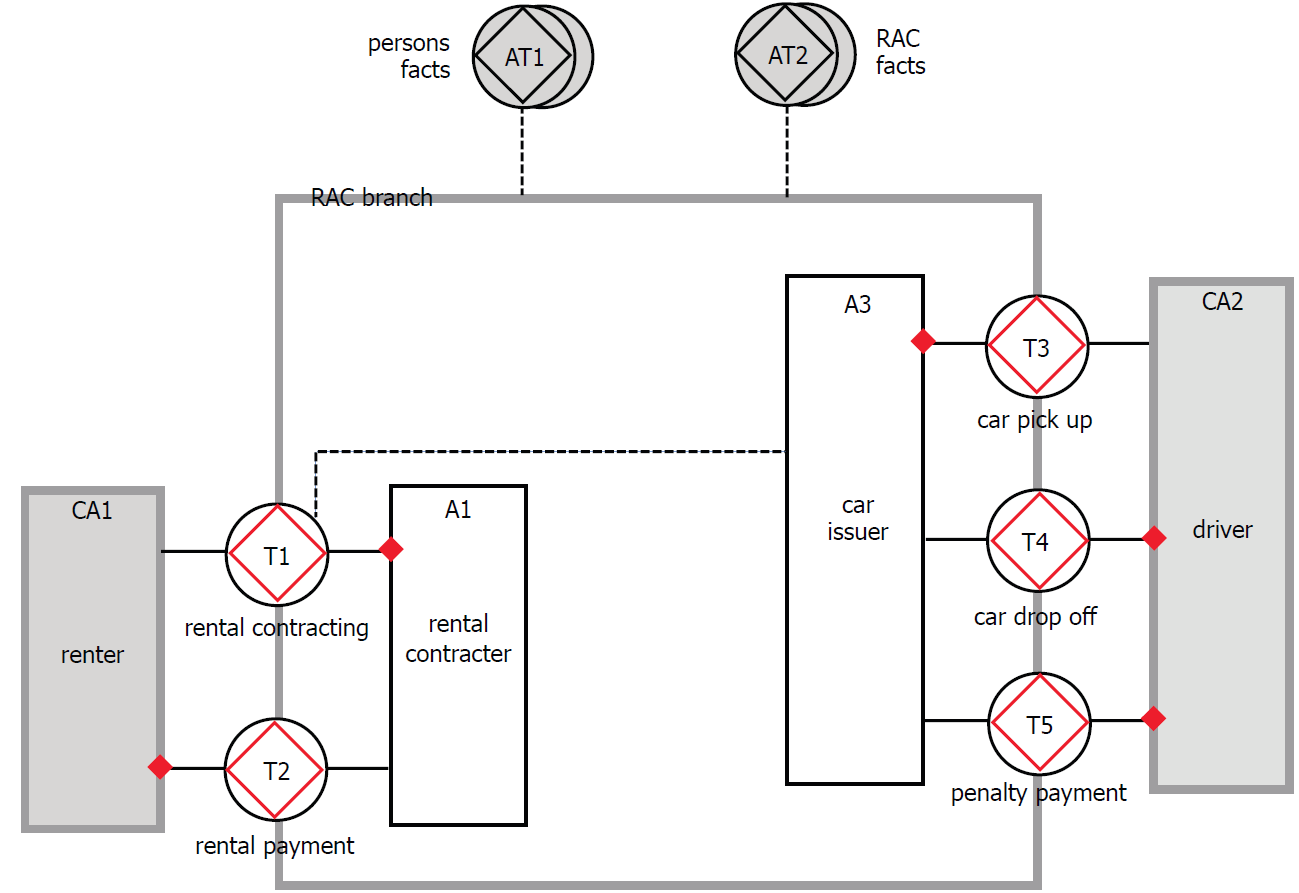
\includegraphics[width=10cm,keepaspectratio]{img/rac-ocd}
\caption{RAC OCD}
\label{fig:rac-ocd}
\end{figure}

\begin{figure}[ht!]
 \centering
 \subfloat{{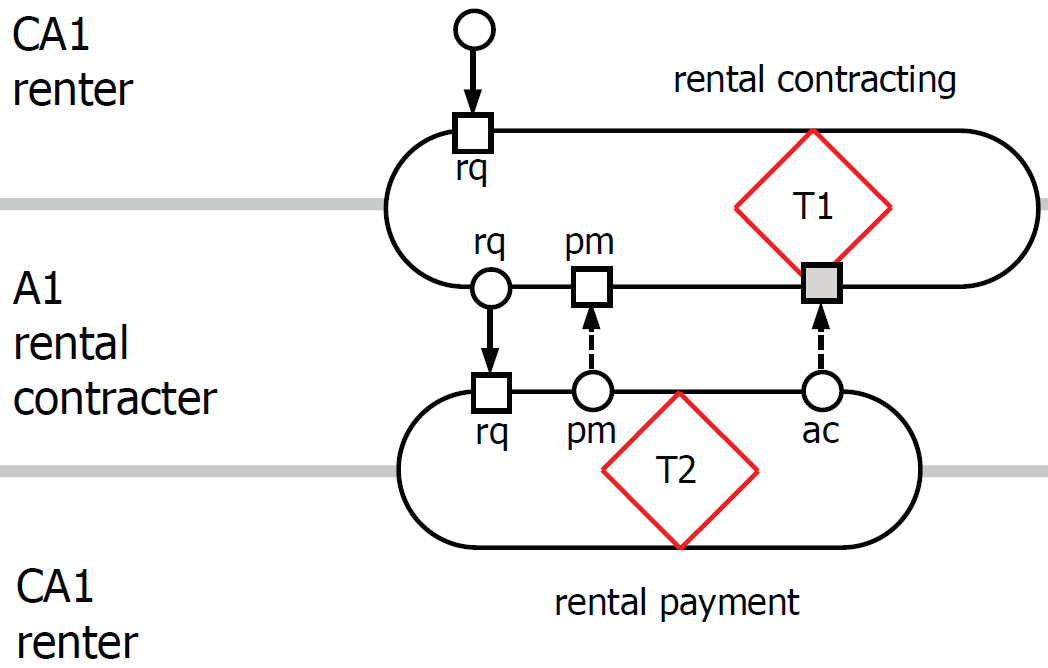
\includegraphics[width=6cm, keepaspectratio]{img/rac-psd-one} }}%
 \qquad
 \subfloat{{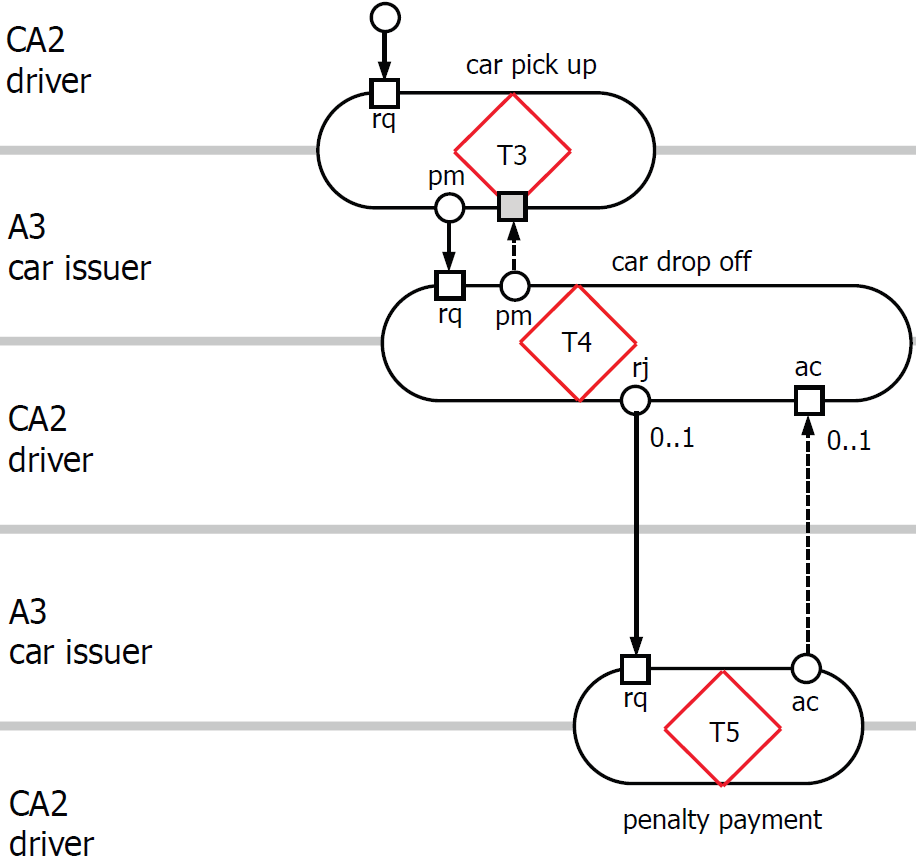
\includegraphics[width=6cm, keepaspectratio]{img/rac-psd-two} }}%
 \caption{RAC PSD}%
 \label{fig:rac-psd}%
\end{figure}
\newpage
% ----------------------------------------------------------------------------------------
\section{Data Labelling}
As has been said, every system within enterprise provides some collection of data. Problem is, if enterprise does note use centralized solution (a some form of \gls{bpms}), format of collected data can be very different. 
However collected data can be structured and then processed via procedure, named ``labelling''. Every system can provide collected data with some structured form. Then sooner defined \textit{Data Aggregation Service} must have mechanism how this structure map to defined \gls{demo} model. This mechanism will be for every enterprise and theirs systems unique, however fundamental idea and work-flow is the same.

Firstly used terms are defined:
\begin{description}
\item[log] -- The structured collected data from enterprise systems
\item[case id] -- The defined process.
\item[creation timestamp] -- Timestamp when created.
\item[end timestamp] -- Indicates end of given task.
\item[activity] -- An activity (task) within case.
\item[resource] -- An resource associated with activity. Typically an user.
\item[role] -- An user role which invoked an activity.
\end{description}

\Cref{tab:rac-log} is an shortened log from \textit{Rent-A-Car} company. The ``case id'' is equal to 1 (which is generally some internal identifier) and it is omitted from table. Also timestamps are omitted because they are not, for now, important.  

There are several activities, resources and roles. ``Labelling'' mechanism must distinguish each one of activities and assign appropriate \textit{Transaction} and \textit{Coordination-act} from \gls{demo} model. Also ``roles'' must be assigned to \textit{Actor roles} and ``resource'' is assigned as \textit{Actor}. An shortened example of ``labelling'' is shown at~\cref{tab:rac-log-labelling}. The ``role'' and \textit{Actor roles} are absolutely the same. 

\begin{table}[ht!]
\centering
\begin{tabular}{ | c | c | c | }
\hline
	\textbf{Activity} & \textbf{Resource} & \textbf{Role} \\ \hline
	Create Rental  Requisition & Peter Freeman & Renter \\ \hline
	Create Request for Payment & Alice Gree & Rental Contracter \\ \hline
	Payment Promise & Peter Freeman & Renter \\ \hline
	Analyse Rental Requisition & Alice Gree & Rental Contracter \\ \hline
	Make a Payment & Peter Freeman & Renter \\ \hline
	Accept Payment & Alice Gree & Rental Contracter \\ \hline
	Create a New Contract & Alice Gree & Rental Contracter \\ \hline
	Hand Over Contract to Customer & Alice Gree & Rental Contracter \\ \hline
	Customer Accepted Contract & Peter Freeman & Renter \\ \hline
	Create Car Pick Up  Requisition & Peter Freeman & Driver \\ \hline
    \multicolumn{3}{|c|}{\dots} \\ \hline
    
% 	Acquire Car Pick Up Request & Bob Hershel & Car Issuer \\ \hline
% 	Create Car Drop Off Requisition & Bob Hershel & Car Issuer \\ \hline
% 	Drop Off Requisition Agreement & Peter Freeman & Driver \\ \hline
% 	Car Preparation & Bob Hershel & Car Issuer \\ \hline
% 	Car Prepared for Pick Up & Bob Hershel & Car Issuer \\ \hline
% 	Driver Acquired the Car & Peter Freeman & Driver \\ \hline
% 	Customer Returning the Car & Peter Freeman & Driver \\ \hline
% 	Customer Returned the Car & Peter Freeman & Driver \\ \hline
% 	Car Returned & Bob Hershel & Car Issuer \\ \hline  
\end{tabular}
\caption{An example log of Rent-A-Car company}
\label{tab:rac-log}
  
\begin{tabular}{ | c | c | c | }
\hline
	\textbf{Activity} & \textbf{Transaction} & \textbf{State} \\ \hline
	Create Rental  Requisition & T1 & Request \\ \hline
	Create Request for Payment & T2 & Request \\ \hline
	Payment Promise & T2 & Promise \\ \hline
	Analyse Rental Requisition & T1 & Promise \\ \hline
	Make a Payment & T2 & State \\ \hline
	Accept Payment & T2 & Accept \\ \hline
	Create a New Contract & T1 & Execute \\ \hline
	Hand Over Contract to Customer & T1 & State \\ \hline
	Customer Accepted Contract & T1 & Accept \\ \hline
	Create Car Pick Up  Requisition & T3 & Request \\ \hline
    \multicolumn{3}{|c|}{\dots} \\ \hline
% 	Acquire Car Pick Up Request & T3 & Promise \\ \hline
% 	Create Car Drop Off Requisition & T4 & Request \\ \hline
% 	Drop Off Requisition Agreement & T4 & Promise \\ \hline
% 	Car Preparation & T3 & Execute \\ \hline
% 	Car Prepared for Pick Up & T3 & State \\ \hline
% 	Driver Acquired the Car & T4 & Accept \\ \hline
% 	Customer Returning the Car & T4 & Execute \\ \hline
% 	Customer Returned the Car & T4 & State \\ \hline
% 	Car Returned & T4 & Accept \\ \hline
\end{tabular}
\caption{Activities labelling from RAC log}
\label{tab:rac-log-labelling}
\end{table}
\clearpage
% -----------------------------------------------------------------------
\section{Process Instance Visualisation}
System must have ability to visualise running process instances in real-time. User can open running process and can be informed how it continues. 

The biggest challenge was how to propose a way to visualise models modelled with \gls{demo}. Moreover, the intent was mainly to provide visualisation on mobile devices (smart-phones, tablets).

There are four conditions how visualisation must be proposed:
\begin{enumerate}[i]
	\item The proposed way must preserve the intention of modelled model through \gls{demo}
    \item Visualisation must be consistent accordingly to defined \gls{demo} model.
    \item The proposed way must be easy to use and understand.  
    \item It must be adaptive to different sizes of mobile devices. 
\end{enumerate}

The first idea of visualisation was highly inspired from investigated existing solutions (\textit{Process Maker}, \textit{Bizagi Modeler}). Visualisation could be done with \gls{demo} \gls{ocd} model itself. With this approach user could have:
\begin{enumerate}
  \item The exactly same understanding of modelled enterprise.
  \item The straightforward visualisation of instances through defined models. If user understand \gls{demo} models, this approach of visualisation has the same meaning.
\end{enumerate}

With this approach first two conditions are accomplished:
\begin{enumerate}
\item Defined enterprise is directly exposed with \gls{ocd} model. However some information are hidden. As is known, the \gls{psd} brings more information how processes are defined and how they work (i). 
\item Consistency is tied with \gls{ocd} itself (ii).
\end{enumerate}

However the (iii) and (iv) are not so straightforward. The third condition (iii) is not accomplished because DEMO is used and it does not have to be easy to use and understand. In every enterprise there are specialists (business analysts) that have the responsibility to analyse given enterprise and specify models (for example within \gls{demo}). Other people do not need to have knowledge about this methodology, overall they do not need to have knowledge about some models either. Although \gls{ocd} itself is very concise, it is not so suitable to smaller screens of mobile devices. This implies, that also (iv) is violated.
% ----------------------------------------------------------------------------------------
\section{A Better Option}
Gantt chart is widely used in time-management projects and systems. It is well known, established and used. It was found, that Gantt chart offers the best approach, how tasks can be visualised. Chosen approach is highly inspired from it and visualisation is based on it. 

The visualisation is divided to two parts:
\begin{enumerate}
\item The ``Gantt-chart canvas'' where each transaction has own form of progress bars which displays transaction's current state.
\item Time-line which offers chronological overview which events occurred and when. 
\end{enumerate}
% ----------------------------------------------------------------------------------------
\subsection{Transaction Box Element}
Transaction box is associated rectangle with transaction which indicates current state of transaction. The state corresponds to actual C-Act within \textit{Transaction Pattern}. Current state also indicates progress value which is displayed as inner rectangle inside transaction box filled with colour. Progress value is computed as percentage value from current state. The C-Act \textit{Request} corresponds to 10 \%, \textit{Promise} to 25 \%, \textit{Execute} to 50 \%, \textit{State} to 75 \% and so on.  

The transaction box has four colour stages. \textbf{White} for not requested transaction yet (the box has also dashed border), a \textbf{green} which indicates ``happy path'' through \textit{Transaction Pattern}, a \textbf{yellow} if transaction is \textit{rejected} or \textit{declined} and \textbf{red} for transaction which is \textit{stopped} or \textit{quitted}. 

The transaction boxes are placed accordingly to \gls{ocd} model. That means:
\begin{itemize}
\item The transaction which ``starts'' whole process is placed as first. 
\item If transaction is dependent on another, it is placed ``under'' it and shifted to the right. Also that means, that ``parent'' transaction is wider than their descendants. 
\end{itemize}
% ----------------------------------------------------------------------------------------
\subsection{Transaction Link Element}
As has been said, \gls{psd} model defines associations between transactions. Each transaction can have many \textit{response} links and \textit{waiting} links. For better understanding, how process is defined, these links are within visualisation included. 

The links appearance is taken from \gls{psd} itself. 
\begin{itemize}
\item Response link is displayed as straight line with arrow at the end. On one side it has circle with \textit{source} C-Act, on the other side with arrow it has square with \textit{target} C-Act.
\item Waiting links is displayed as response link, but line between is dashed. 
\end{itemize}

Links are placed between appropriate transactions accordingly to \textit{source} and \textit{target} C-Acts, just like at \gls{psd}. However, if \textit{response} link has \textit{target} C-Act as ``Requested'', the abbreviation of \textit{target} is omitted and link itself is displayed as angled arrow which points to ``start'' of \textit{target} transaction. It is totally clear, that this type of response means exactly ``If given C-Act at  source transaction occurred then target transaction is also requested''.

Example shown at \cref{fig:box-state-state} means exactly: ``When transaction T1 is \textit{promised}, T2 is \textit{requested}. Then T1 can be \textit{stated} only if T2 was already \textit{promised}. Also T1 can be \textit{accepted} only if T2 was \textit{stated}.''

\begin{figure}[ht!]
\centering
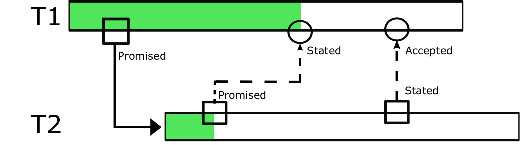
\includegraphics[width=9cm,keepaspectratio]{img/box-links-example}
\caption{The transaction links example}
\label{fig:box-state-state}
\end{figure}

On the canvas's left side are placed transaction labels. Label corresponds to transaction's name and identifier. The labels are structured to tree-form like in folder explorer. Each transaction box has same height position as corresponding label. 

With this approach, user has quick and easy way how can check state of concrete process. User can easily determine which transactions are not yet completed and how they are connected  together. 

However the time-based information still missing and that is the point, where time-line comes in.
% ----------------------------------------------------------------------------------------
\subsection{Time-line}
Main purpose of time-line is to provide chronological overview of incoming events. The time-line is scalable. This means, that user can zoom in or out to level of details. Typically more events can occur within one minute, so it is important to have ability to zoom to more detailed view. 

Each event is marked with timestamp (when event occurred) and what kind of event it is. If event is kind of ``C-Act occurred'', event has also information about associated transaction with C-Act's abbreviation. To help user more easily distinguish which transaction is associated with given event, each transaction has own colour, that is reflected to colour of text within time-line. 

Time-line is independently controllable and provide another point of view to the state of current running process. 

One note aside, the first idea was to provide connected associations between time-line and transaction boxes. The intent was to provide visuals (anchors) within transaction box that could indicate that ``at this point something happened''. If the user `click'' on this anchor then a visual connection between anchor and associated event within time-line appears. 

With this approach, the canvas must be capable of responding to time-line ``stretching'' -- transaction box must resize accordingly to positions of events within time-line. Although it makes perfectly sense from user ``point-of-view'', the usability within mobile-devices is reduced. Each event within time-line must be readable and with adding of events, width of transaction box grows. Result is, that each transaction box is really wide and it becomes very unclear and nearly unusable.

Result is that, the visualisation is divided to two views. First one, the time-line offer chronological overviews of occurred events associated with transactions. The second one offers the overview current transactions states and the associated links between them. 

The earlier four defined conditions for visualisation are fully accomplished.

\begin{enumerate}[i]
	\item \begin{graytext}
    ``The proposed way must preserve the intention of modelled model through \gls{demo}''\end{graytext}
    
    The defined model through \gls{demo} is displayed within \textit{Gantt-chart canvas}. \gls{ocd} is transformed to \textit{transaction boxes} and \gls{psd} is transformed to \textit{transaction links}.
    \item \begin{graytext}``Visualisation must be consistent accordingly to defined \gls{demo} model.`` \end{graytext}
    
    The \gls{ocd} model is transformed to another form on view, but the name of transactions and associations between them remains. The links from \gls{psd} are taken as they are, without any significant changes.
    \item \begin{graytext}``The proposed way must be easy to use and understand.''\end{graytext}
    
    As has been said, the Gantt charts are well known and many people on management positions or analysts naturally understand to this concept of views. The \textit{transaction boxes} easily  show current state of given transaction and \textit{transaction links} show associations between them.    
    \item \begin{graytext}``It must be adaptive to different sizes of mobile devices.''\end{graytext}
    
    The time-line part is perfectly adaptive to various screen sizes. The ``Gantt-chart canvas'' is more concise than more larger \gls{ocd} and it can more easily adapt to smaller screens.
\end{enumerate}

% ----------------------------------------------------------------------------------------
\section{The Dashboard}
Although the ``process visualisation'' brings usable kinds of overviews, there are many types of overviews which can't be done through this. As has been said in \cref{ch:bpms}, typical \gls{bpm} solutions offers some kind of ``dashboard'' where these various types of overviews are placed together. 

The dashboard's main goal is to provide:
\begin{enumerate}
\item The comprehensive and effective way how to get precious information over collected data.
\item Ability to provide highly customized and individual types of overviews. A company will want to propose a different overviews for sales manager than for accountant and so on. 
\item The overviews must be easy to understand and must be very clear, what they display.
\end{enumerate}

\subsection{Data Query}
To provide a specific view over collected data, it is required to collected data be specifically aggregated according to defined overviews. For this purpose, the \textit{data query} is defined.

\textit{Data Query} is basically named query over collected data. This also can be also compared as ``stored-procedure'' within DBMS (Database Management System). From end-user point of view, user only select defined query and data are returned. Within \textit{Data Aggregation Service} query is defined and transformed to ``real'' query over collected data. In most of cases, it will be transformed to SQL-like query. 

Within \gls{bpm} solution (based on \gls{demo}) is defined \textit{query editor}. It is simple, form-based editor, where employees within an enterprise can define \textit{data queries}. User defines \textit{name} of query and builds the query with interactive guide. For simplicity, the guide can be imagined as interactive way how to build a SQL query with clauses as ``join, where, group by, order by, etc.''. Result is, that editor allows to non-technical users still define basic queries over collected data without requirement to have knowledge, how concretely ``grab'' the data in technical way. An example of query editor (as prototype) is shown at \cref{fig:query-editor}.

\begin{figure}[ht!]
\centering
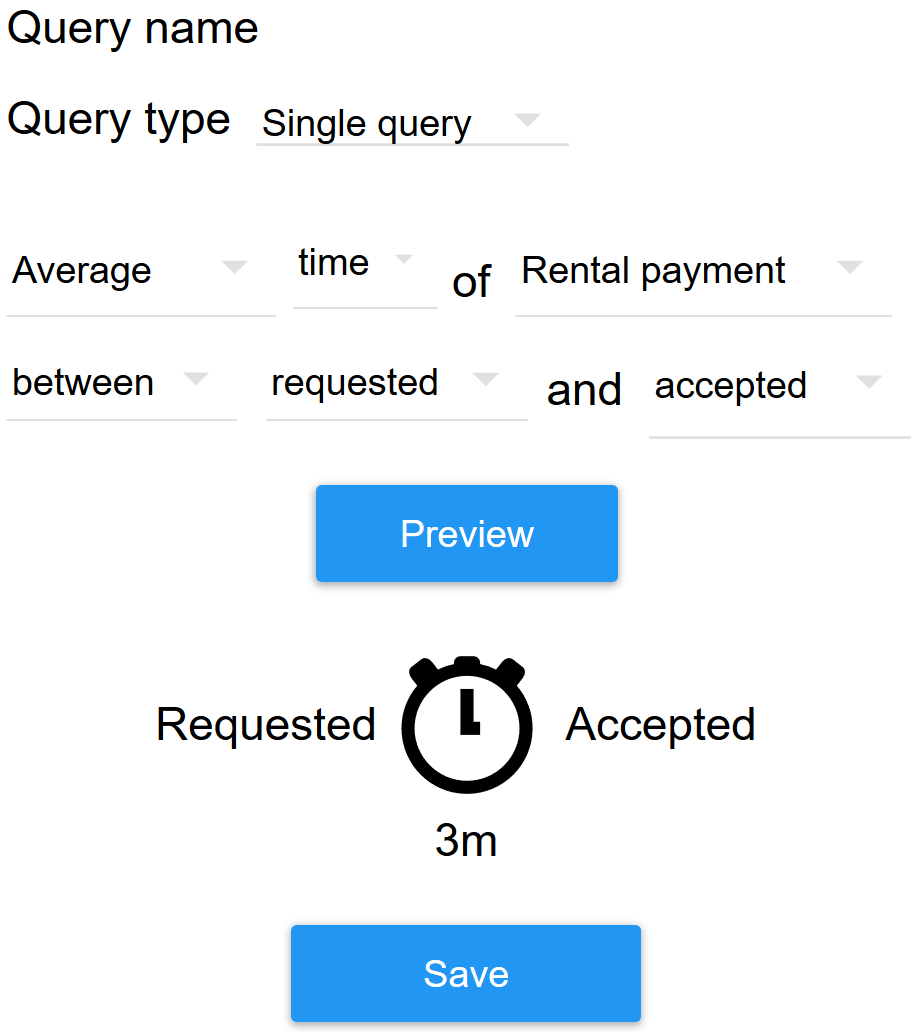
\includegraphics[width=6cm,keepaspectratio]{img/query-editor}
\caption{The Query editor prototype example}
\label{fig:query-editor}
\end{figure}

Each overview within dashboard is called \textit{widget}. Widgets provide one concrete type of view. Widgets has defined \textit{name} and associated \textit{data query}. Each widget is highly customisable, but they are sorted to a several base types.

\subsection{Summary Widget}
The summary widget provides, by its name, summarization about collected data. It is commonly displayed as ``Pie chart''. The typical usage for example can be: ``Summary of ratio between Accepted and Declined contracts'' or ``Actual state of all contracts, number of requested, stated, declined, accepted and so on'',~\dots

\subsection{Time Based Widget}
This widget displays data between defined time period. It uses ``Column chart''  (each \textit{time x-value} is displayed as column with height of \textit{y-value}) or ``Line series chart''. An example of typical usage can be: ``Monthly income-expense'', ``Daily number of new contracts'',~\dots

\subsection{Single Value Widget}
An single value computed from collected data. This can be for example ``Actual number of unresolved contracts'', ``Actual financial balance'',~\dots 

\subsection{Widgets As Placeable Elements}
Dashboard can be divided to ``grid layout'' -- a unspecified number of rows and from one up to three columns. Each widget has defined the \textit{width} and the \textit{height} -- how many columns and rows it will take. The the user can simply arranges widgets exactly how he wants.


\section{\todo{Graphs as Widgets, Dashboard}}
\section{\todo{Queries and editor}}
\section{\todo{A Few More Ideas of Visualisation}}
%     \section{Overviews}
    
%     \section{Process visualization}
    
%     \section{Mobile application concept}
	
% 	\todo{Domain model of collected data. Proposed way of real time visualization. Type of charts. Dashboard. Whole concept of application, e.g dashboard, editor. Functional specification, a.k.a example use cases?? Domain model of collected data.}
    
%     \section{Analysis}    

   

% 	\section{The dashboard}
%     Purpose of dashboard is provide centralized overview of processes such as average waiting time before process is completed or total amount of requests per day. The appearance of dashboard depends on user. \gls{dwma} provides customizable elements called widgets to achieve desired look for every user individually.

%     \subsection{Widgets}  
%      Widgets are small independent configurable components for displaying collected data from business processes. Each one has purpose. Notice that widgets are only user-friendly view of query above collected data. For editing widgets there is widget editor. User can simply edit properties of widget such as name, category, tags and of course source of data - the query and second important property is the type of widget. There are following types of widgets:
     
%      \textbf{The summary widget} (\cref{fig:widget-summary}) provides, by it's name, chart with summarization of collected data. Concrete type of the chart depends on the user and on the data. Summary widget provides several types of charts:
     
%      \begin{enumerate}
%     	\item \textit{Pie} chart is used to illustrate numerical proportion.         
%         \item  \textit{Bar} chart displays categorical data with numerical value.
%         %\item \textit{Line}
%     \end{enumerate}
      
%       \begin{figure}[ht!]
%           \centering
%           
\includegraphics[width=6cm,keepaspectratio]{img/TODO-image}
%           \caption{Summary widget example}
%           \label{fig:widget-summary}
%       \end{figure}   
    
%    	Second type is \textbf{Time period} (\cref{fig:widget-time-period}). Time period displays data in some interval. Typically it can serve as overview \textit{``Number of requests for Rental payment per day"}.        
      
%       \begin{figure}[ht!]
%           \centering
%           
\includegraphics[width=6cm,keepaspectratio]{img/TODO-image}
%           \caption{Time period widget example}
%           \label{fig:widget-time-period}
%       \end{figure}
    
%     Last type is \textbf{Single query} (\cref{fig:widget-single-query}) which allows display simple result from query. Prerequisite for query is that query returns one single record. 
      
%       \begin{figure}[ht!]
%           \centering
%           
\includegraphics[width=6cm,keepaspectratio]{img/TODO-image}
%           \caption{Single query example}
%            \label{fig:widget-single-query}
%       \end{figure}       
    
%     \subsection{Query editor}
    
%     \todo{Information about query editor}
    
%     \begin{figure}[ht!]
%           \centering
%           
\includegraphics[width=6cm,keepaspectratio]{img/TODO-image}
%           \caption{\todo{Query editor}}
%       \end{figure}   
    
%     \section{The real-time overview of process instance}
%     \todo{Introduction about gantt chart. Make conversation about classic OCD / PSD diagrams and their pros and cons for visualizations}
%     Provides the real-time overview of one concrete process instance.
% On the left side is tree-view (like in folder explorer) of transactions. Each transaction has identifier and name.
% On the top is the timeline which displays important events from the process. Above timeline is visualization itself. Each transaction is displayed as progress bar with some visual tweak, which will be discussed later.

% 	Each transaction can be at one of the following state, which has different visual: 
% 	\todo{Categories}
    
%     \begin{description}
%     	\item[Not active transaction] Is displayed as greyed out progress bar. It means that this instance of transaction will be probably started at some future time.

%         \item[Active transaction] Progress bar is displayed with green colour to show current progress of instance transaction. 
        
%         \item[Completed transaction] Progress bar is fulfilled with green colour. It means that given transaction successfully ended (was accepted).
        
%         \item[Stopped transaction] Progress bar changed colour to red which indicates that transaction failed to complete due to fact that it was quitted or stopped. 
%     \end{description}
    
%  \subsection{Response and waiting links}
%     \todo{Change this}
%    Each transaction can have several child-transactions and also many conditional links. These conditions are displayed with arrows pointed to another transaction with the condition.
% Conditions are divided into two categories.

% If the condition is ``Some state of transaction A has to be done before transaction B can start (be requested)", e.g. transaction A must be stated before transaction B can be requested (\cref{fig:request-start-condition}).

% \begin{figure}
%   \centering
%   
\includegraphics[width=6cm,keepaspectratio]{img/TODO-image}
%   \caption{\todo{Request-start condition}}
%   \label{fig:request-start-condition}
% \end{figure}  

% If condition is ``Some state of transaction A has to be done before transaction B can be at another state", e.g transaction A must be at least stated before transaction B can be promised (\cref{fig:state-state-condition}).

% \begin{figure}
%   \centering
%   
\includegraphics[width=6cm,keepaspectratio]{img/TODO-image}
%   \caption{\todo{State-state condition}}
%   \label{fig:state-state-condition}
% \end{figure}  

